% Template for a Computer Science Tripos Part II project dissertation
\documentclass[12pt,a4paper,twoside,openright]{report}
\usepackage[utf8]{inputenc}
\usepackage[pdfborder={0 0 0}]{hyperref}    % turns references into hyperlinks
\usepackage[margin=25mm]{geometry}  % adjusts page layout
\usepackage{graphicx}  % allows inclusion of PDF, PNG and JPG images
\usepackage{verbatim}
\usepackage{docmute}   % only needed to allow inclusion of proposal.tex
\usepackage[utf8]{inputenc}
\usepackage{mathtools}
\usepackage{changepage}
\usepackage{url}
\usepackage{blindtext}
\usepackage{amssymb}
\usepackage{xcolor}
\usepackage{bbm}
\usepackage{bm}
\usepackage[
backend=biber,
style=ieee,
sorting=none
]{biblatex}
\addbibresource{references.bib}

\newcommand{\suploss}{\mathcal{L}^\text{sup}}
\newcommand{\clsloss}{\mathcal{L}^\text{class}}
\newcommand{\regloss}{\mathcal{L}^\text{reg}}


%\raggedbottom                           % try to avoid widows and orphans
\sloppy
\clubpenalty1000%
\widowpenalty1000%

\renewcommand{\baselinestretch}{1.1}    % adjust line spacing to make
                                        % more readable

\begin{document}
% Change these

\newcommand{\mcandidate}{123456}
\newcommand{\mfullname}{Martin Richards}
\newcommand{\mcollege}{St John's College}
\newcommand{\mtitle}{How to write a dissertation in \LaTeX}
\newcommand{\mexamination}{Computer Science Tripos -- Part II}
\newcommand{\mdate}{July, 2001}
\newcommand{\moriginator}{Dr M.~Richards}
\newcommand{\msupervisor}{Dr Markus Kuhn}
\newcommand{\mwordcount}{1587}
\newcommand{\mlinecount}{1000}
% Consent to the dissertation made available to University members
\newcommand{\mconsent}{I am content for my dissertation to be made available to the students and staff of the University.}
% For the Declaration of originality
\newcommand{\msignature}{Full Name Here}




%%%%%%%%%%%%%%%%%%%%%%%%%%%%%%%%%%%%%%%%%%%%%%%%%%%%%%%%%%%%%%%%%%%%%%%%
% Title


\thispagestyle{empty}

\rightline{\LARGE \textbf{\mfullname}}

\vspace*{60mm}
\begin{center}
\Huge
\textbf{\mtitle} \\[5mm]
\mexamination \\[5mm]
\mcollege \\[5mm]
\mdate  % today's date
\end{center}

%%%%%%%%%%%%%%%%%%%%%%%%%%%%%%%%%%%%%%%%%%%%%%%%%%%%%%%%%%%%%%%%%%%%%%%%%%%%%%
% Proforma, table of contents and list of figures

\pagestyle{plain}

\newpage
\newpage
\section*{Declaration of originality}

I, \mfullname{} of \mcollege, being a candidate for Part II of the Computer Science Tripos, hereby declare that this dissertation and the work described in it are my own work, unaided except as may be specified below, and that the dissertation does not contain material that has already been used to any substantial extent for a comparable purpose. \mconsent

\bigskip
\leftline{Signed \texttt{\msignature}}
\bigskip
\leftline{Date \today}

\chapter*{Proforma}

{\large
\begin{tabular}{ll}
Candidate Number:   & \bf \mcandidate                   \\
Project Title:      & \bf \mtitle                       \\
Examination:        & \bf \mexamination, \mdate         \\
Word Count:         & \bf \mwordcount\footnotemark[1]   \\
Code Line Count:    & \bf \mlinecount                   \\
Project Originator: & \bf \moriginator                  \\
Supervisor:         & \bf \msupervisor                  \\ 
\end{tabular}
}
\footnotetext[1]{This word count was computed
by \texttt{detex diss.tex | tr -cd '0-9A-Za-z $\tt\backslash$n' | wc -w}
}
\stepcounter{footnote}


\section*{Original Aims of the Project}
% At most 100 words



\section*{Work Completed}
% At most 100 words

All that has been completed appears in this dissertation.

\section*{Special Difficulties}
% At most 100 words
None.

\newpage

\tableofcontents

\listoffigures

\newpage
\section*{Acknowledgements}


\pagestyle{headings}

\chapter{Introduction}

\chapter{Preparation}

\section{Background}
In the interest of brevity, this section assumes a fundamental understanding of concepts related to deep learning such as neural networks, backpropagation, and gradient descent. Greater effort is made to explain concepts relevant to the core requirements of this project.

\subsection{Convolutional neural network}
Convolutional Neural Networks (CNNs) are a type of deep learning algorithm that uses \textit{Convolution} operations. CNNs are particularly suitable for image and video analysis as they preserve the spatial structure of multi-dimensional data. A CNN model usually contains multiple convolutional layers. In each convolutional layer, a fixed size \textit{kernel} is trained. During the forward pass, the kernel is applied across the dimensions of the input data, regardless of its size. This allows \textit{fully-convolutional CNN models}, which consists of exclusively convolutional layers, to handle input of variable sizes.

\subsection{Object detection}
Object detection consists of two separate tasks:
\begin{itemize}
    \item \textbf{Detection.} Identifying the location of objects in the input image. The output of this task is usually a bounding box around each detected object, or a mask that isolates the object from the background (segmentation).
    \item \textbf{Classification} Assigning each detected object into a set of classes. The output of this task is typically a score that indicate how confident is the model that a particular object belongs to a particular class.
\end{itemize}

Differences in how these two tasks are handled inspired two different approaches to object detection: \textbf{two-stage} and \textbf{one-stage}.

\subsubsection{Two-stage object detection}
Two-stage object detection models handles detection first, followed by classification. For example, the Faster-RCNN model consists of a Region Proposal Network (RPN) for detection and a deep neural network (DNN) for classification. For each image, the RPN produces a set of bounding boxes that could contain detections. Region of Interest (RoI) pooling layer is used to convert variable-size features into fixed-size features, which can then be fed to the DNN classifier.

\subsubsection{One-stage object detection}
One-stage detection models handle detection and classification simultaneously. A typical one-stage object detection model shares the vast majority of its convolutional layers for both classification and detection. The output from these shared layers passes through separate classification and detection networks simultaneously

\subsubsection{Comparison}
In terms of time of publication, two-stage object detectors have a head start with the publication of R-CNN \cite{girshick_rich_2014} in 2014. R-CNN is subsequently improved by Fast R-CNN \cite{girshick_fast_2015} in 2015, then by Faster R-CNN \cite{ren_faster_2016} and Mask R-CNN in 2017. One-stage object detectors becomes mainstream with the publication of YOLO (You Only Look Once) \cite{redmon_you_2016} in 2016, which has spawned a series of incrementally improved variants that are still being published.

In general, two-stage object detectors offer better performance. However, the simplicity of the one-stage detectors allows them to be significantly more efficient. In recent years, the continuous refinement of one-stage detection has narrowed the performance gap.

As the aim of this project is to achieve efficient detection, I will be using EfficientDet \cite{tan_efficientdet_2020}, a one-stage object detection architecture published in 2020.

\subsection{Supervised Contrastive Learning}
Contrastive learning is a deep learning learning method that aims to learn representations of data that capture underlying patterns and similarities. The idea is to pull together `positive' samples in embedding space, while pushing apart `negative' samples. By maximising the similarity between similar pairs and minimising the similarity between dissimilar pairs, contrastive learning enables the discovery of useful features that can be applied to downstream tasks such as image classification and object detection.

Applying this technique to supervised learning, supervised contrastive loss \cite{khosla_supervised_2021} maximises similarity between samples from the same class while minimising similarity between samples from different classes. 

For a batch of samples with embeddings $\{\mathit{z}_1, \dots, \mathit{z}_n\}$ and label $\{y_1, \dots, y_n\}$. Supervised contrastive loss is defined as:
\begin{align}
    A(i) &= \{a \in [1,n]\ |\ a \neq i\}\\
    P(i) &= \{p \in A(i)\ |\ y_p = y_i\}\\
    \suploss &= \sum\limits_{i\in [1, n]}\suploss_i=\sum\limits_{i\in [1, n]}\frac{-1}{|P(i)|}
    \sum\limits_{p\in P(i)}\log\frac{\exp{(\mathit{z}_i \bullet \mathit{z}_p})}{\sum\limits_{a \in A(i)}\exp{(\mathit{z}_i \bullet \mathit{z}_a)}} \label{eq:supcon}   
\end{align}
$A(i)$ includes all samples except $i$ while $P(i)$ includes all samples that have the same class as $i$ except $i$ itself. $\bullet$ is the dot product. Minimising $\suploss$ maximises cosine similarity between same-class embeddings and minimises the cosine similarity between different-class embeddings.

\subsubsection{Supervised contrastive learning for object detection}
While supervised contrastive learning has been successfully applied for object classification \cite{khosla_supervised_2021} and NLP tasks \cite{gunel_supervised_2021}, I could find very little literature about applying supervised contrastive learning for object detection. As far as I am aware, this project is the first attempt to use supervised contrastive learning for a one-stage object detection model.

\section{Requirements}
The main objective of the project is to implement software that detects and classifies deep-sea organisms from input video footage. Based on the requirements set out in the project proposal, the project consists of three core requirements.
\begin{itemize}
    \item Implement the EfficientDet object detection model
    \item Implement supervised contrastive loss for EfficientDet
    \item Implement software that mixes creatures and backgrounds from different images to create new training examples
\end{itemize}

\subsection{Risks}
I used the Cambridge High Performance Computing (HPC) cluster for model training and other computation-intensive parts of this project. This introduces several risks:
\begin{itemize}
    \item Learning curve of HPC
    \item Unforeseen bugs when running code on HPC, the difficulty of remote debugging
    \item Long queue time resulting in delay in project
\end{itemize}
To mitigate the first factor, I read the HPC documentation and learnt through trial and error with small test jobs. To mitigate the second factor, I wrote unit tests for every critical components of the project. After every major change, I requested interactive sessions from the HPC cluster to test and debug in real time. These measures helped minimise wasted training time, which also mitigates the third factor. As a backup, I could train my model on my laptop or on a commercial compute platform like AWS Sagemaker.

\section{Software Engineering}
In this section, I will analyse the software engineering techniques and tools that I used to complete this project.

\subsection{Language \& Frameworks}
I wrote the project in Python as it is the language-of-choice for Machine Learning tasks. I chose to build my deep learning models on PyTorch, as it has excellent documentation, community support, and a suite of debugging tools. For computer vision related tasks, I used both OpenCV and Pillow, as I required different features from them. For hyperparameter tuning, I chose Optuna as it is well-documented, light-weight and feature-rich. 

\subsection{Version Control}
I used Git for version control with a repository on GitHub. I used the Google Drive Windows client to maintain a backup of my entire development environment. 

\subsection{Tests}
I used PyTest for all unit tests in this project and integrated it with GitHub Actions to run the unit tests after every commit. I learnt from this project that it is very easy to introduce bugs with vectorised operations. Thus, I rewrote critical components in plain Python and tested for consistency between the two implementations.

ML models proved difficult for testing as I often do not know the correct output. I used Neptune to produce model data flow diagrams and analysed them manually for consistency. When possible, I also tested models by loading pretrained parameters from other implementations, which helps to ensure correct parameter dimensions. 

\section{Starting Point}
This project drew significant inspiration from Garðar Ingvarasson's Part II project from 2021-2022. Garðar implemented a Faster R-CNN deep-sea organism detector and trained it on the same dataset as mine. Nonetheless, this project is implemented completely independently. I only referenced Garðar's code on two occasions:
\begin{enumerate}
    \item I compared Garðar's evaluation code to mine to ensure they are consistent. This is to establish a fair basis of comparison between our models.
    \item I tested the model size of Garðar's model for the sake of comparison.
\end{enumerate}
I will elaborate more on these in the evaluation chapter.

Prior to this project, I had used python for several personal projects and are comfortable with the language. Regarding object detection, I used a command-line utility to train an object detection model in TensorFlow. However, the utility used was very high level and there was barely any coding involved. My only other prior experience with machine learning frameworks was completing several TensorFlow and PyTorch tutorials.

\chapter{Implementation}
\section{Repository Overview}
\section{Dataset}

I trained and evaluated the models of this projects on the FathomNet \cite{katija_fathomnet_2022} dataset.

WRITE MORE!
\subsection{Dataset Breakdown}
\begin{center}
    \begin{tabular}{||c c||}
    \hline
     \textbf{Object Class} & \textbf{\# Annotations}  \\
     \hline
     \hline 
     Black corals & 261\\
     Demosponges & 1057 \\
     Glass sponges & 3291 \\
     Sea anemones & 7920 \\
     Sea cucumbers & 6409 \\
     Sea pens & 3871 \\
     Sea pigs & 8304 \\
     Sea urchins & 14164 \\
     Soft corals & 8402 \\
     Starfish & 7066 \\
     Stony corals & 130 \\
     \hline
    \end{tabular}
\end{center}

\section{Training Example Generator}
In this following sections, I will cover how I created a algorithm that generates new training examples from the existing dataset. The main methodology of the algorithm can be summarised as ``crop out creatures and paste them to new background''. While it is easy to understand, getting the entire algorithm to work required the many distinct software components, which I will cover in details.

\subsection{Creature Extraction}
The first step of this process is to extract creatures from their backgrounds. 
At first, the only reliable way to extract creatures was to do so manually. I built an iterative algorithm using GrabCut \cite{rother_grabcut_nodate} to make this process more efficient. At the start of each iteration, I manually drew hints to GrabCut about which parts of the image are backgrounds and foregrounds. The GrabCut algorithm uses these hints to improve its foreground segmentation. Using this algorithm, I am usually able to extract a suitable crop in 3 iterations. In total, 500 creatures were manually cropped from the images using this method.

\subsection{Creature transformations}
To make the most of the extracted creatures, I designed transformations that can be applied to individual creatures to create many more examples.

\subsubsection{Horizontal Flip}
This transform applies a horizontal flip to a creature. As virtually all creatures in my dataset are roughly left-right symmetrical, this is almost always a reasonable transform.

\subsubsection{Rotation}
This transformation rotates a creature by an angle sampled from a truncated normal distribution. The parameters of the transform controls the truncated normal distribution.

\subsubsection{Scale}
This transformation scales the creature in the X and Y axis. The extent of the scaling is determined by two factors sampled from a truncated normal distribution. Similar to rotation, this transform's parameters are those of its probability distribution.

\subsubsection{Perspective}
This transformation applies random translations to the four corners of creature's image, then maps the original image so that it fits within quadrilateral formed by these new corners. Its parameters control the extent of the corners' translation.

\subsubsection{Distort}
This transformation is derived from an algorithm designed to remove lens distortion. It first finds a random point in the image of the creature. It then either distorts the image around the chosen point. Its parameters control how the random point is generated and the extent of the distortion.

\subsubsection{Transformation pipeline}
These transformations are combined into a transformation pipeline. With the help of Dr Emily Mitchell, I tuned custom transformation pipelines tailored for different classes of organisms. For easy modifications, transformation pipelines could be constructed from JSON configuration files.


\subsection{Creature Location Generation}
The next step in the generation process is to find locations in existing images where the new creatures may be added. When I wrote the project proposal, I only considered the possibility of pasting creatures into ``empty'' regions of existing images. I later discovered that replacing creatures in the image is also a viable alternative, with both methods offering pros and cons.

\subsubsection{Pasting}
In each background image, proposal boxes, bounding boxes where new creatures could be placed, are generated . The size and aspect ratio of the proposal boxes are randomly sampled from bounding boxes from the entire dataset. A newly generated proposal boxes must not overlap with creature labels or older proposal boxes, otherwise they will be discarded. From empirical observations, it is generally not advisable to paste new creatures near the top of images. This is because these regions are often above the sea floor where no organism in this project could be found. Therefore, an additional rule states that the upper edge of proposal boxes must be below the highest upper edge of all labelled creatures.

\subsubsection{Replacement}
With replacement, the first step is to remove the existing creature from the image. Image inpainting techniques can be applied to hide the empty space left behind by the removed creature. Among many options, I settled on the inpainting technique proposed by Telea \cite{telea_image_2004}, which is implemented in the OpenCV library.A major drawback of replacement is when the region to be inpainted is large, inpainting can become expensive and inevitably leaves noticeable visual artefacts. 

\subsubsection{Trade-offs}
Pasting offers greater efficiency at the risk of adding creatures to unsuitable locations. Replacement will always place creatures at suitable locations, but is computationally more expensive and does not scale well to large creatures. With this trade-off in mind, I decided to use both techniques simultaneously, preferring pasting for larger creatures and replacement for smaller creatures.

\subsection{Matching}
At this stage, I have a set of potential locations where new creatures could be added and a set of cropped creatures that can be added. The next step is to match each potential location with a suitable cropped creature.

I considered the following factors during the matching process:
\begin{itemize}
    \item \textbf{Pixel dimensions}. It is undesirable to stretch a low resolution cropped creature over a large area. It may be more acceptable to shrink a higher resolution cropped creature to fit into a smaller space.
    \item \textbf{Aspect ratio}. A similar aspect ratio is needed to prevent excessive stretching.
    \item \textbf{Relative size in image}: This measures how much of an image does a creature/space occupy. 
\end{itemize}

Using these factors, I assign probability scores to potential cropped creatures, which are then used to sample the final cropped creature from the pool.

\subsection{Extension: ML Generation of Creature Crops}
As an extension task, I trained a Generative Adversarial Network (GAN) that learnt to generate cropped creatures. Instead of implementing a GAN from the ground up, I used the Mimicry \cite{lee_mimicry_2020} library, which is created in a past Part II project supervised by my supervisor, Dr Chris Town. For the model architecture, I chose to use InfoMax-GAN, which was proposed in the same Part II project.

During training, my creature augmentation pipeline is used for data augmentation. 
......
\subsection{Extension: Creature Segmentation}

.....


\section{EfficientDet}
EfficientDet \cite{tan_efficientdet_2020} is a one-stage object detection model published in 2020. It is based on EfficientNet \cite{tan_efficientnet_2020-1}, an image classification model published in 2019. Similarly to EfficientNet, EfficientDet makes use of a single integer scaling factor that scales different dimensions of the model. Neural architectural search was used to maximise EfficientDet's performance within limited compute budgets. At the time of publications, EfficientDet outperformed many object detection models despite having much fewer weights and lower computational cost.

\subsection{Architecture}
In this section, I will cover the major components of EfficientDet and explain how it is used for detection and classification.

\begin{figure}[h]
    \centering
    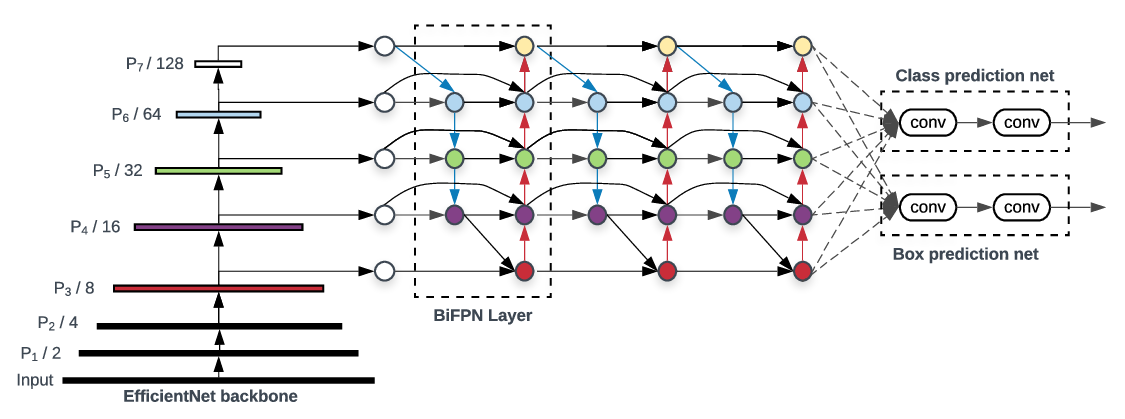
\includegraphics[width=0.9\textwidth]{figs/implementation/efficientdetarch.png}
    \caption{EfficientDet architecture}
    \label{fig:efficientdetarch}
\end{figure}

\subsubsection{EfficientNet backbone}
An input image is first passed through an EfficientNet \cite{tan_efficientnet_2020} backbone. In EfficientNet, the output of the final convolutional layer is passed to a DNN classifier to produce one class prediction for the entire image. In EfficientDet however, outputs at selected convolutional layers are extracted into a stack of feature maps at different resolutions. We call this multi-resolution stack a \textit{feature pyramid}. 

\subsubsection{Bi-directional Feature Pyramid Network (BiFPN)}
\begin{figure}[h]
    \centering
    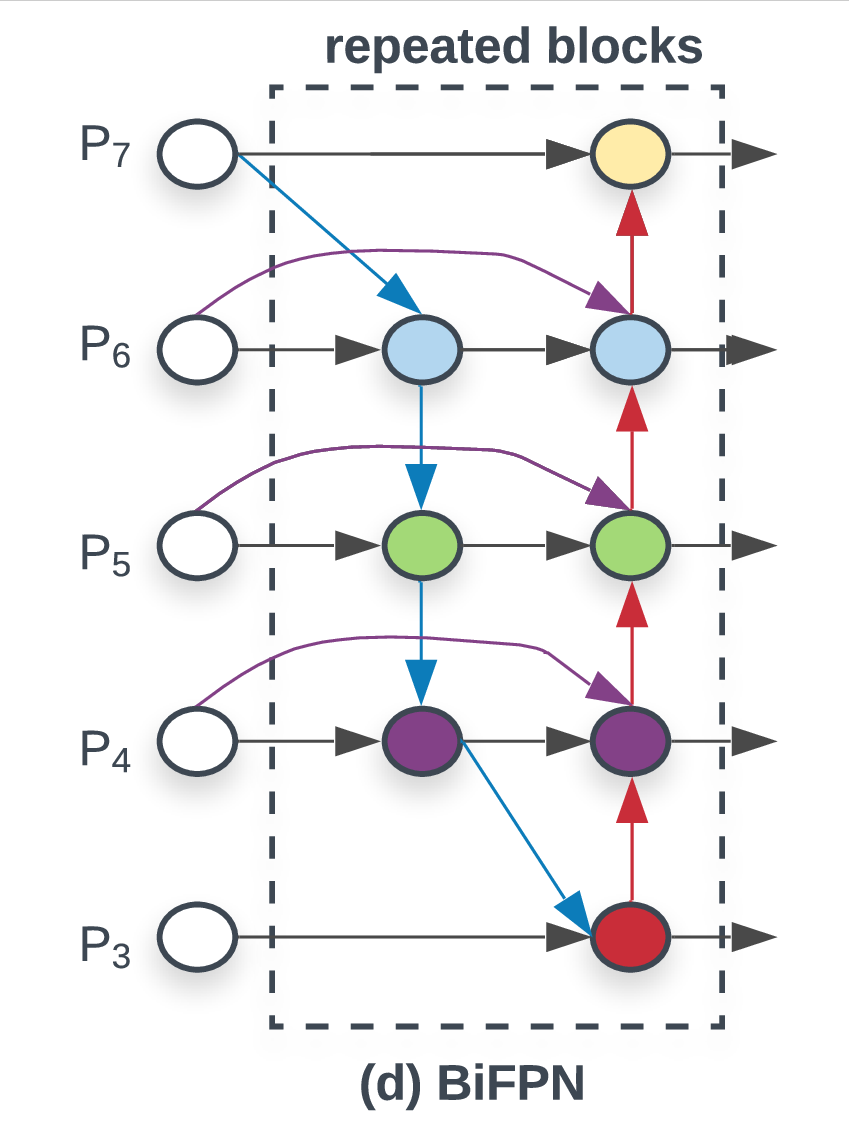
\includegraphics[height=5cm]{figs/implementation/bifpn.png}
    \caption{Components of one BiFPN layer: \textcolor{cyan}{$\rightarrow$} indicates nearest neighbour upsampling, \textcolor{red}{$\rightarrow$} indicates max pooling downsampling, \textcolor{purple}{$\rightarrow$} indicates $1\times 1$ convolution}
    \label{fig:bifpn}
\end{figure}

The BiFPN inputs and outputs feature pyramids. The goal is to aggregate features at different resolutions to create semantically meaningful features. When combining features of different resolutions are combined, BiFPN takes a weighted sum of input feature maps.
\begin{align}
    O=\sum_i \frac{w_i}{\epsilon + \sum_j w_j}\cdot I_i
\end{align}
Where $I_i$ are input features and $O$ is the output feature; $w_i$ are learned weights for each input feature map, and $\epsilon$ is used to ensure numerical stability.

\subsubsection{One-stage detection and classification}
EfficientDet uses feature pyramids for both detection and classification. A feature pyramid is a stack of feature maps of different dimensions. A feature map is a tensor of shape $H \times W \times D$, which corresponds to the height, width and feature depth. Let's refer to each $1\times 1\times D$ section of the feature map as a grid cell. Each grid cell corresponds to a region of the input image. For example, if a $2\times 2 \times 16$ feature map is derived from a $512 \times 512$ input image, each grid cell corresponds to a $256 \times 256$ region in the input image. For each grid cell, its $D$-length feature vector should be a semantically meaningful representation of its corresponding region of the input image. 

EfficientDet uses the BiFPN grid cell features for both detection and classification. Each cell of the grid is associated with multiple detections through \textit{anchor boxes}. Anchor boxes are predefined bounding boxes which are placed relative to the centre of each grid cell. In EfficientDet, each grid cell is associated with $A=9$ anchor boxes, a Cartesian product of 3 scales and 3 aspect ratios. 

An anchor box is a single unit of detection and classification. During training, labels are assigned to each anchor box based on the maximum Intersection over Union (IoU) value between the anchor box and any ground truth bounding box. When maximum IoU $> 0.5$, the anchor box is matched and  should produce the same class and bounding box as the maximum ground truth. When maximum IoU $< 0.4$,  the anchor box is assumed to be unmatched; it should predict a low confidence score for every class and will not contribute to the detection loss. In between, the anchor box is considered too ambiguous and will contribute to neither classification nor detection loss.

EfficientDet uses two separate CNN modules to for detection and classification. The two modules share a common architecture, the only difference being the output shape of the final layer. 

\begin{figure}[h]
    \centering
    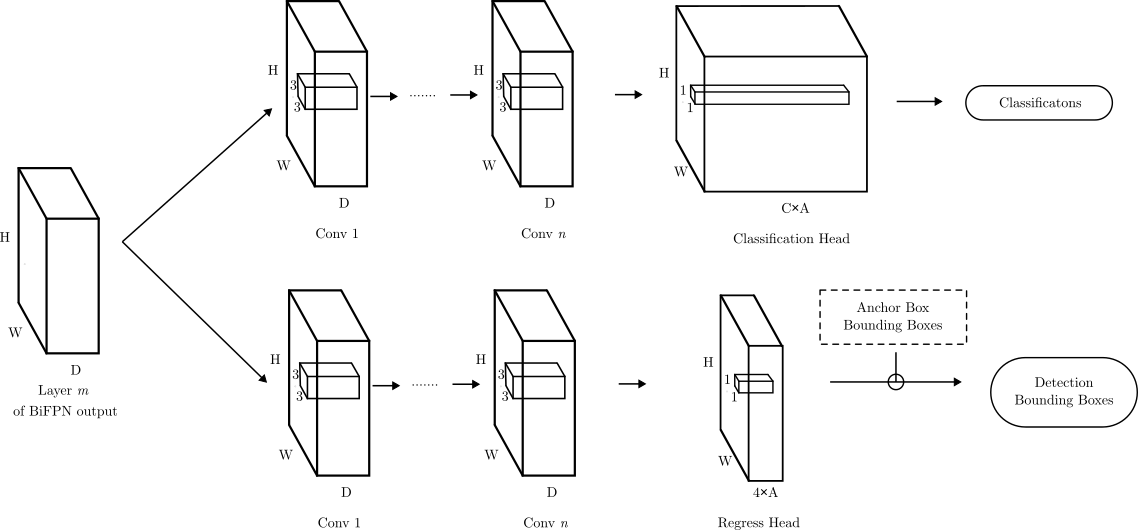
\includegraphics[width=0.9\textwidth]{figs/implementation/efficientdet_heads.png}
    \caption{\textbf{EfficientDet Detection and Classification Architecture}: The detection and classification modules branches off from BiFPN output.}
    \label{fig:edet_heads}
\end{figure}
\subsubsection{Box prediction net}
For every anchor box, the detection module is trained to predict 4 transform parameters that map the anchor box bounding boxes to the ground truth bounding boxes. 

\subsubsection{Class prediction net}
For every anchor box, the classification module is trained to predict a confidence score for every class. The sigmoid function $S(x)=\frac{1}{1+e^{-x}}$ is applied on module output to squash the output between 0 and 1. Note that softmax is not used here as the model is trained to represent ``No object detected'' by predicting a low confidence score for every class.

\subsection{Losses}
\subsubsection{Detection: Smooth L1 Loss}
For regression loss, EfficientDet uses Smooth L1 loss. For prediction $x$ and truth $y$, Smooth L1 loss is defined as: 
\begin{align} \label{eq:smooth_l1}
    \regloss = \begin{cases}
        \frac{1}{2\beta}(x-y)^2\quad\ \text{if } |x-y| < \beta\\
        |x-y|-\frac{1}{2\beta}\quad \text{otherwise}
    \end{cases}
\end{align}

\subsubsection{Classification: Focal Loss}
For classification loss, EfficientDet uses Focal Loss \cite{lin_focal_2018} proposed in 2017. Focal Loss downweighs the contribution of easy examples on the total classification loss. This helps to focus training on difficult examples. Focal loss is controlled by the parameter $\gamma$. The greater the value of $\gamma$, the greater the skew introduced by focal loss. If $p$ is the model's estimated probability and $y$ is the label, focal loss is defined as:


\begin{align}\label{eq:focal}
p_t&=\begin{cases}
    p\quad\quad\text{if }y=1\\
    1-p\ \text{otherwise}
    \end{cases}\\
\clsloss &= -(1-p_t)^\gamma \log(p_t)
\end{align}
When $\gamma=0$, the focal loss becomes $-\log(p_t)$, which is equivalent to cross-entropy loss.

\subsubsection{Total loss}
Combining the detection and classification losses, we derived a formula for the total loss of EfficientDet:
$$
\mathcal{L}^{\text{total}} = \clsloss + \kappa\regloss
$$
 Where $\kappa$ is a tuned hyperparameter. 

\subsection{Implementation}
Before starting to implement EfficientNet and EfficientDet, I read both research papers thoroughly. For details not covered in the research paper, I consulted the official TensorFlow implementations of the models. For reference during the implementation process, I sketched the architecture of both models on my iPad and annotated the sketches with details I picked up while reading the source code. As this is my first time implementing a model in PyTorch, I followed PyTorch tutorials on custom CNN models and read through best practises for writing PyTorch modules.

The subtle differences between TensorFlow and PyTorch proved to be a major challenge for me. For example, the official EfficientDet implementation uses convolutional layers that preserves input/output dimensions despite the use of custom kernel sizes. This can be achieved with one extra argument in TensorFlow; it is not straightforward in PyTorch....

\section{Supervised Contrastive Learning}
In the following section, I will detail my experiment to implement supervised contrastive loss \cite{khosla_supervised_2021} for object detection.

\subsection{Problem Analysis}
The problem of porting supervised contrastive loss to EfficientDet boils down to two important questions:
\begin{enumerate}
    \item \textit{What are the object features?}\\ 
    Recall that supervised contrastive learning aims to maximise similarity between features of similar concepts while minimising the similarity between different concepts. In this context, concepts refer to the labelled objects in the images. To implement supervised contrastive loss, I need to derive features for every labelled object.

    EfficientDet provides `grid cell' features that correspond to different regions of the image. How do I transform these features into object features?
    \item \textit{How do I train with contrastive loss?}\\
    Supervised contrastive loss \cite{khosla_supervised_2021} is proposed for the one task of image classifications. Object detection requires training for both detection and classification tasks. How should I mix both tasks at training time?
\end{enumerate}

\subsection{First failed attempt}
\subsubsection{Object features by summing grid cell features}
In EfficientDet, grid cell features capture meaningful information about regions of the input image. I thought a viable way to derive object features is by taking a weighted sum of grid cell features based on how much the object overlaps with the corresponding regions.

I used IoU to determine whether an object should be associated with a grid cell. For grid cells $c_1, \dots, c_n$, let $A(i)$ be the set of anchor boxes for grid cell $c_i$. The correspondence $K(j, i)$ between object $o_j$ and grid cell $c_i$ is defined as:
\begin{align}
    K(j, i) &= \frac{1}{|A(i)|}\sum\limits_{a\in A(i)} \text{IoU}(o_j, c_i)
\end{align}

I determined the weight between grid cells and objects using the inverse of the catesian distance between their center points, denoted by $d_{x, y}$. The weight between object $o_j$ and grid cell $c_i$ is defined as:
\begin{align}
    w(j, i) = \mathbbm{1}_{K(i,j)>0} \cdot \frac{1}{(d_{j, i})^2}
\end{align}

For grid cell features $\bm{f}_i, \dots, \bm{f}_n$, the object feature $\bm{x}_j$ of $o_j$ is defined as:
\begin{align}
    \bm{x}^*_j &= \sum\limits_{i\in 1\dots n} w(j, i) \cdot \bm{f}_i \\
    \bm{x}_j &= \frac{\bm{x}^*_j}{||\bm{x}^*_j||^2}
\end{align}

\subsubsection{Projection network}
Instead of computing similarity between concept features directly, modern contrastive learning techniques often first passes the concept features through a small \textit{projection network}. The output projections are normalised and used to calculate similarity. 

I decided to emulate the original Supervised contrastive learning paper \cite{khosla_supervised_2021} and used a Multi-Layer Perception (MLP) with one hidden-layer for my projection network. The dimension of the projection network, $\mathcal{D}^p$, is a tuned hyperparameter. The projection network is discarded after training.

\subsubsection{Two stage training}
The original Supervised contrastive learning paper \cite{khosla_supervised_2021} used a two-stage training methodology. In the first stage, the model is pretrained on contrastive loss. between the stages, all model weights are frozen except for the final linear classifier. In the second stage, the linear classifier is trained on the traditional classification task. Their results show that after 700 epochs of first-stage contrastive training, only 10 epochs of training was needed for the second stage.

For my first attempt, I decided to follow this technique as closely as possible. Specifically, I trained the model in two stages using the following losses:

\begin{align*}
    \textbf{Stage 1: }& \suploss\\
    \textbf{Stage 2: }& \clsloss + \kappa \regloss
\end{align*}

Note that the second stage loss function is equivalent to the total loss function of EfficientDet. Thus, this training methodology essentially adds supervised pretraining on top of EfficientDet.

\subsection{Results and Reflections}
Despite many my best effort, I was unable to get the design described to work. Contrastive loss usually stops decreasing within 20 epochs of training. When fed to the second training stage, the pretrained models failed to outperform randomly initialised models. It is clear that my methodology failed to learn effective representations for creatures in the dataset.

\subsubsection{Potential causes of failure}
In this section, I note several potential reasons which I think led to the failure.
\begin{enumerate}
    \item Shifting anchor boxes. In training, EfficientDet learns to transform anchor boxes to fit object bounding boxes. As a result, the region covered by each anchor box changes during training. The previous design assumes static anchor box positions through out, potentially limiting performance.
    \item Low batch size. The original supervised contrastive loss \cite{khosla_supervised_2021} is trained with a batch size of 6144, with the author recommending a batch size above 2048. I could only achieve a maximum batch size of 110 with distributed training over 4 GPUs on the Cambridge HPC. As supervised contrastive loss consider similarities within each batch, batch size likely has a large impact on training convergence.
    
\end{enumerate}

\subsubsection{Reflections}
To address the first potential cause, instead of basing object feature calculation on static anchor boxes, I could base it on the trained transformed anchor boxes. This is most effective when contrastive loss and detection loss are trained simultaneously.

The second potential cause makes me consider the realistic possibility that pretraining on contrastive loss could take too long to complete. This could cause severe delays in project progress and deplete limited server time. In the interest of risk mitigation, I decided that it was prudent to abandon the technique.

\subsection{Second Attempt}

\subsubsection{Object features with dynamic detection boxes}
An input image is first passed through EfficientDet to produce transformed anchor boxes. For each labelled object, we find the $K$ transformed anchor boxes with the highest IoU values. The object feature is the normalised weighted sum of the $K$ anchor box features. The weight assigned to each anchor box feature is inversely proportional to the rank of the anchor box, raised to the power $\rho$. 
\begin{align}
    \bm{f}^*(o_i) &= \sum\limits_{i\in [1,K]}\frac{\bm{f}(a_{\text{TopK}(o_i)[i]})}{i^\rho}\\
    \bm{f}(o_i) &= \frac{\bm{f}^*(o_i)}{||\bm{f}^*(o_i)||^2}
\end{align}


\subsubsection{Anchor box features}

\begin{figure}[h]
    \centering
    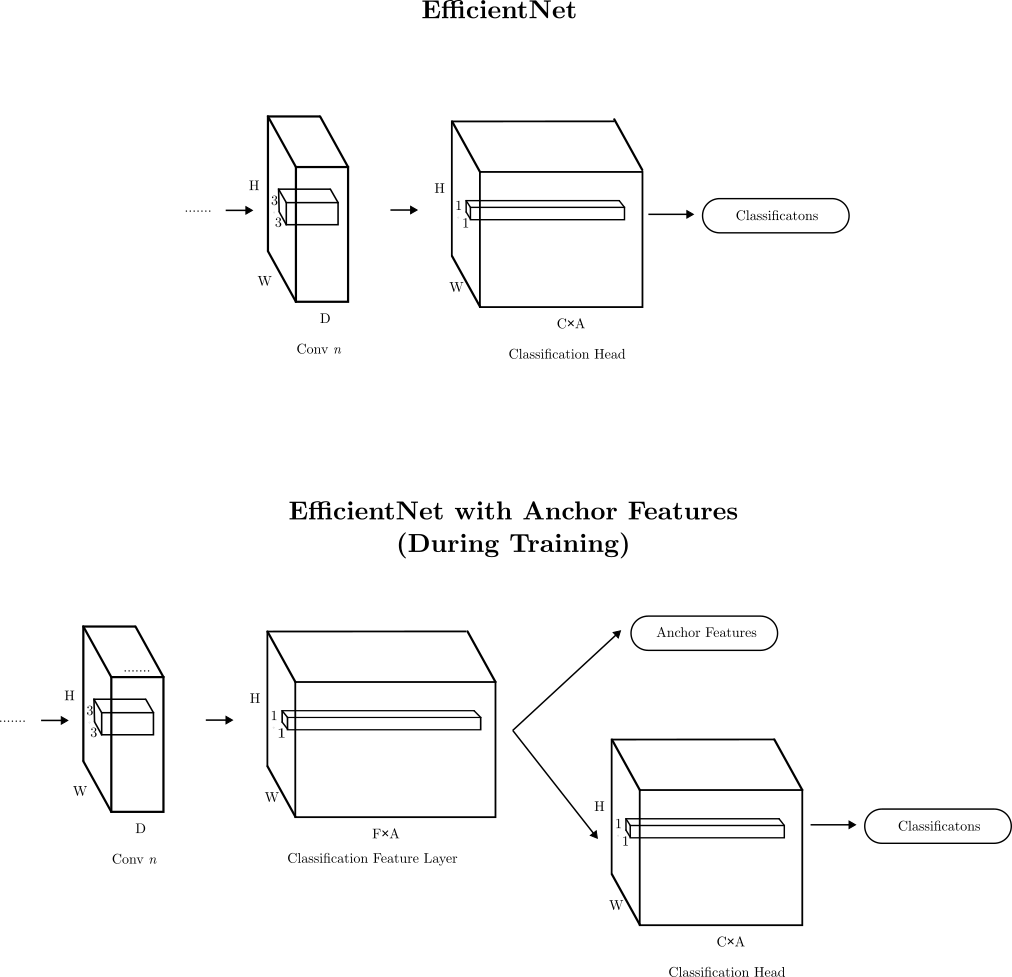
\includegraphics[width=0.8\textwidth]{figs/implementation/efficientdet_new_head.png}
    \caption{\textbf{EfficientDet for Anchor Features: }During training, the final $1\times 1$ convolutional layer is replaced by two layers in order to extract anchor box features for contrastive loss.}
    \label{fig:edet_new_head}
\end{figure}
The previous section covers a new object feature formula, which requires features for each anchor box. However, EfficientDet only produces features for each grid cell. To derive anchor box features from grid cell features, I propose a modification to the final classification layer of EfficientDet at training time. Instead of one $1\times 1$ convolutional layer with $(D, C\times A)$ input/output channels, two $1\times 1$ convolutional layers are used with $(D, F\times A)$ and $(F\times A, C\times A)$ input/output channels respectively.  The output of the first convolutional layer is used as anchor box features. $F$ is the number of element in each anchor box feature. 

A key advantage of this design is that it does not modify EfficientDet after training, as the two $1\times 1$ convolutional layers can collapse into a single $1\times 1$ convolutional layer. 

\subsubsection{One stage training}
A new one-stage training methodology with loss function will be used:
$$
\clsloss + \kappa \regloss + \lambda \suploss
$$
$\lambda$ is a new tuned hyperparameters.

\section{Training \& Hyperparameter Tuning}
\chapter{Evaluation}


\chapter{Conclusions}

I hope that this rough guide to writing a dissertation is \LaTeX\ has
been helpful and saved you time.


%%%%%%%%%%%%%%%%%%%%%%%%%%%%%%%%%%%%%%%%%%%%%%%%%%%%%%%%%%%%%%%%%%%%%
% the bibliography
\addcontentsline{toc}{chapter}{Bibliography}
\printbibliography[
heading=bibintoc,
title={Bibliography}
]

%%%%%%%%%%%%%%%%%%%%%%%%%%%%%%%%%%%%%%%%%%%%%%%%%%%%%%%%%%%%%%%%%%%%%
% the appendices
\appendix
\end{document}